
\documentclass{article}
\usepackage{titletoc}

\usepackage{geometry}
\geometry{
    a4paper,
    total={170mm,257mm},
    left=20mm,
    top=20mm,
}

\newcommand*{\template}{../dding_template}

\input{\template/tex_packages/tex_packages_general.tex}
\input{\template/tex_macros/tex_macros_general.tex}
\usepackage{appendix}

\dottedcontents{section}[2em]{\bfseries}{1.5em}{1pc}
\dottedcontents{subsection}[3em]{}{1.7em}{1pc}

% \newtheorem{remark}{Remark}[section]
% \newtheorem{assum}{Assumption}[section]
% \newtheorem{lem}{Lemma}[section]
% \newtheorem{theorem}{Theorem}[section]
% \newtheorem{prop}{Property}[section]
% \theoremstyle{definition}
% \newtheorem{definition}{Definition}[section]

% ========================================
\newcommand*{\bdx}{\mv{x}} % bold x
\newcommand*{\bdy}{\mv{u}} % bold u
\newcommand*{\bdz}{\mv{z}} % bold z
\newcommand*{\bdq}{\mv{q}} % bold q

\newcommand*{\bdf}{\mv{f}} % bold f

\newcommand*{\tpfpx}{\pptfrac{\bdf}{\bdx}} % partial f / partial x
\newcommand*{\pfpx}{\ppfrac{\bdf}{\bdx}} % partial f / partial x

\DeclareMathOperator{\sym}{sym}
% ========================================

\title{
    Deep-Neuro Control with Contraction Theory
}
\author{Myenogseok Ryu, Sesun You}
\date{20\textsuperscript{th} March 2025}

\begin{document}

\maketitle

\begin{abstract}
    This project aims to develop control or estimator with deep neural network and contraction theory.
\end{abstract}

\tableofcontents

\section{Introduction}

\subsection{Motivation}

\subsection{Literature Review}

\section{Notations and Preliminaries}

The following notations are used throughout this document:
\begin{itemize}
    \item $:=$ denotes \textit{defined as}.
    \item $(\cdot)^\top$ denotes the transpose of a matrix or a vector.
    \item $\bdx:=[x_i]_{i\in\{1,\cdots,n\}}\in\R^n$ denotes the state vector.
    \item $\mm A:=[a_{ij}]_{i,j\in\{1,\cdots,n\}}\in\R^{n\times n}$ denotes a matrix.
    \item $\lambda_{i}(\mm A),\ i\in\{\max,\min\}$ denotes the maximum and minimum singular value of $\mm A$, respectively.
    \item $\mm I_n$ denotes the identity matrix of size $n$ and $\mm 0_{n\times m}$ denotes the zero matrix of size $n\times m$.
    \item $\sym$ denotes the symmetric part of a matrix, \ie $\sym(\mm A):=\mm A+\mm A^\top$ \cite{Tsukamoto:2021ac}.
\end{itemize}

We introduce the following lemmas.

\begin{lem}[Comparison Lemma]
	Suppose that a continuously differentiable function $f:\R^n\to\R$ satisfies the following inequality:
	\begin{equation}
		\ddtt f(t)\le -a f(t)+ b, \quad \forall t\in\R_{\ge 0}
		,
	\end{equation}
	where $a,b>0$.
	Then, the following inequality holds:
	\begin{equation}
		f(t)\le -af(0)e^{-at} + \tfrac{b}{a}(1-e^{-at}), \quad \forall t\in\R_{\ge 0}
	\end{equation}
	and remains in a compact set $f(t)\in\{\norm{f(t)} \mid \norm{f(0)}\le \tfrac{b}{a}\}$.
	\label{lem:comparison}
\end{lem}

\begin{proof}
	This is a simple special case of the comparison lemma \cite[pp. 102-103]{Khalil:2002aa}.
	See \cite[pp. 659-660]{Khalil:2002aa}.
\end{proof}

\section{Review of Contraction Theory}

For your smooth start, we recommend you to begin with \cite{LOHMILLER:1998aa}.

\subsection{Basic Results of Contraction Theory for Deterministic Systems}

First, we start with the following deterministic systems:
\begin{equation}
    \ddtt{\bdx}
    = 
    \bdf(\bdx,t)
    ,
    \label{eq:sys}
\end{equation}
where $\bdf(\bdx,t)$ is an $n\times1$ sufficiently smooth non-linear vector function and $\bdx\in\R^n$ is the state vector.
The smooth property of $\bdf(\bdx,t)$ is essential to ensure the existence and uniqueness of the solution to \eqref{eq:sys} \cite[see, pp. 88-89]{Khalil:2002aa}.

\begin{figure}[!ht]
    \centering
    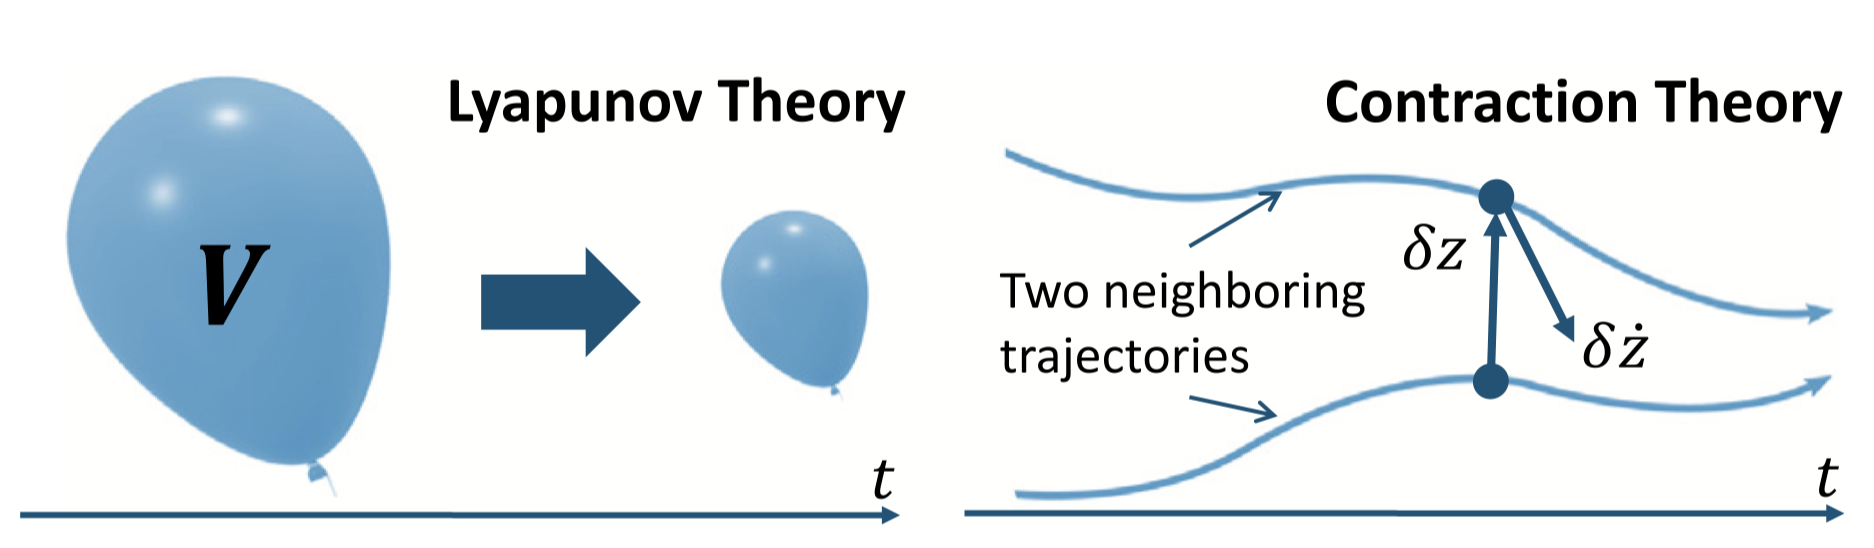
\includegraphics[width=0.5\textwidth]{figs/lyaVSctrac.png}
    \caption{
        Difference between Lyapunov and contraction theory \cite[Fig. 1]{Tsukamoto:2021aa}.
        The Lyapunov theory investigates the convergence to a single point and the contraction theory does regarding a single trajectory.
    }
    \label{fig:lyaVSctrac}
\end{figure}

The biggest difference between the traditional Lyapunov theory and the contraction theory is that the contraction theory investigates the convergence of the state trajectory to a single trajectory (contraction behavior), while the Lyapunov theory focuses on the convergence of the state trajectory to a single point \ie see, Fig.~\ref{fig:lyaVSctrac}.
For this, motivated by the calculus of variations \cite[Chap. 4]{Kirk:2004aa}, \eqref{eq:sys} can be rewritten as differential dynamics using \textit{differential displacement} $\delta\bdx$ as follows:
\begin{equation}
    \ddtt\delta\bdx
    =
    \tpfpx(\bdx,t)
    \delta\bdx.
    .
    \label{eq:diff_sys}
\end{equation}
For your information, $\delta\bdx$ is an infinitesimal displacement at \textit{fixed time}.

\subsubsection{Notable Definitions}

Before we present the fundamental theorem of contraction theory, we introduce the following definitions.
One can re-visit this section while reading further.

\begin{definition}[see, Def. 2.2 \cite{Tsukamoto:2021aa}]  
    If any two trajectories $\mv\xi_1(t)$ and $\mv\xi_2(t)$ of \eqref{eq:sys} converge to a single trajectory, then the system \eqref{eq:sys} is said to be \textit{incrementally exponentially stable}, if $\exists C,\alpha>0$, subject to the following holds:
    \begin{equation}      
        \norm{\mv\xi_1(t)-\mv\xi_2(t)}
        \le 
        C
        \norm{\mv\xi_1(0)-\mv\xi_2(0)}
        \exp^{-\alpha t}
        ,\ \forall t\in\R_{\ge 0}
        .
    \end{equation}
    The result of Theorem \ref{thm:ctrac:main} equivalently implies the incremental exponential stability, since we have $\norm{\mv\xi_1(t)-\mv\xi_2(t)}= \norm{\int_{\mv\xi_1(t)}^{\mv\xi_2(t)}\delta\bdx(t)}$.
    \label{def:inc_exp_stable}
\end{definition}

\begin{definition}
    Let $\mm\Theta(\bdx,t)$ be a smooth coordinate transformation of $\delta\bdx$ to $\delta\bdz$, \ie $\delta\bdz = \Theta(\bdx,t)\delta\bdx$.
    Then, a symmetric continuously differentiable matrix $\mm M(\bdx,t):=\mm\Theta(\bdx,t)^\top\mm\Theta(\bdx,t)$ is said to be a \textit{metric} of the system \eqref{eq:sys}.
    \label{def:metric}
\end{definition}

\begin{definition}
    The covariant derivative of $\mv f(\bdx,t)$ in $\delta\bdx$ coordinate is represented as 
    \begin{equation}
        \mm F
        :=
        \left(
            \ddtt\mm\Theta
            +
            \mm\Theta\tpfpx
        \right)
        \mm\Theta^{-1}
        ,
    \end{equation}
    and is called the \textit{generalized Jacobian}.
    This can be easily derived by differentiating $\delta\bdz = \Theta(\bdx,t)\delta\bdx$ with respect to $t$.
\end{definition}

\subsubsection{Notable Theorems}

The following theorem is the fundamental theorem of contraction theory.
\begin{theorem}[see, T. 2.1 \cite{Tsukamoto:2021aa}]
    If $
        \exists \mm{M}(\bdx,t)
        =
        \mm\Theta(\bdx,t)^\top
        \mm\Theta(\bdx,t)
        > 0, \forall \bdx,t
    $ where $\mm\Theta(\bdx,t)$ defines a smooth coordinate transformation of $\delta\bdx$ to $\delta\bdz$, \ie $\delta\bdz = \Theta(\bdx,t)\delta\bdx$, subject to the following equivalent conditions holds for $\exists\alpha\in\R_{>0},\ \forall \bdx,t$:
    \begin{subequations}
        \begin{align}
            \lambda_{\max} (
                \mm F(\bdx,t)
            )
            =
            \lambda_{\max} 
            \left(
                \left(    
                \ddtt \mm\Theta
                +
                \mm\Theta\tpfpx
                \right)
                \mm\Theta^{-1}
            \right)
            \le&
            -\alpha
            ,
            \\
            \ddtt \mm M
            +
            \sym(\mm M\tpfpx)
            \le&
            -2\alpha\mm M
            ,
        \end{align}
    \end{subequations}
    where the arguments of $\mm M(\bdx,t)$ and $\mm F(\bdx,t)$ are omitted for simplicity, then, the system \eqref{eq:sys} is said to be contracting with an exponential rate $\alpha$, \ie all trajectories of \eqref{eq:sys} converge to a single trajectory.
    The converse is also true.
    \label{thm:ctrac:main}
\end{theorem}

\begin{proof}

\end{proof}

\subsection{Basic Results of Contraction Theory for Stochastic Systems}

\section{Deep-Neuro Control}


\begin{appendices}

\section{Notable Lemmas}

\end{appendices}

\bibliographystyle{ieeetr}
\bibliography{\template/refs}
\end{document}